\chapter{TINJAUAN PUSTAKA}
\label{chap:tinjauan-pustaka}

% Ubah bagian-bagian berikut dengan isi dari tinjauan pustaka

Demi mendukung penelitian ini, \lipsum[1][1-5]

\section{Hasil Penelitian Terdahulu}

Beberapa penelitian terdahulu yang relevan dengan topik ini antara lain \lipsum[1][1-5]

\setlength{\LTpre}{6pt}
\setlength{\LTpost}{6pt}
\begin{longtable}{|c|p{4cm}|p{8cm}|}
  \caption{Penelitian Terdahulu}\label{tab:penelitian-terdahulu} \\
  \hline
  \textbf{No} & \textbf{Penelitian} & \textbf{Pembahasan} \\
  \hline
  \endfirsthead

  \multicolumn{3}{c}{\tablename\ \thetable\ -- \textit{Lanjutan dari halaman sebelumnya}} \\
  \hline
  \textbf{No} & \textbf{Penelitian} & \textbf{Pembahasan} \\
  \hline
  \endhead

  \hline
  \endfoot

  \hline
  \endlastfoot

  1 & Voyager & \parencite{wang2023voyager} \lipsum[2][1-3] \\
  \hline
  2 & Model Context Protocol & \parencite{cilacap2024mcp} \lipsum[2][1-3] \\
  \hline

\end{longtable}

\section{Roket Luar Angkasa}
\label{sec:roket-luar-angkasa}

% Contoh input gambar
\begin{figure}[H]
  \centering

  % Ubah dengan nama file gambar dan ukuran yang akan digunakan
  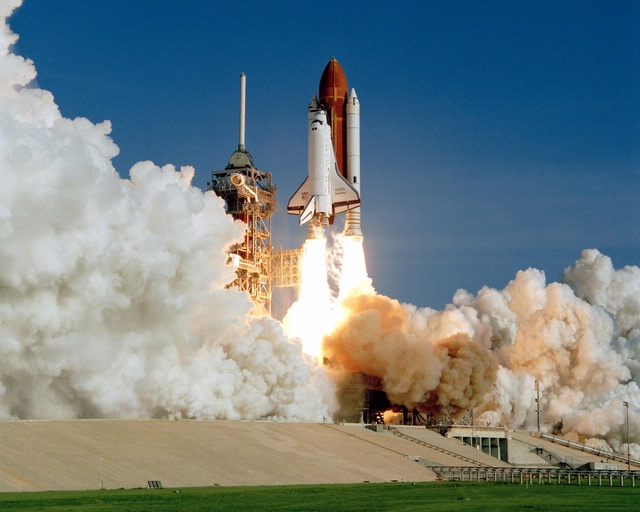
\includegraphics[scale=0.35]{gambar/roketluarangkasa.jpg}

  % Ubah dengan keterangan gambar yang diinginkan
  \caption{Peluncuran roket luar angkasa \emph{Discovery} \parencite{roketluarangkasa}.}
  \label{fig:roket-luar-angkasa}
\end{figure}

Roket luar angkasa merupakan \lipsum[1]

\emph{Discovery}, Gambar \ref{fig:roket-luar-angkasa}, merupakan \lipsum[2]

\section{Gravitasi}
\label{sec:gravitasi}

Gravitasi merupakan \lipsum[1]

\subsection{Hukum Newton}
\label{subsec:hukum-newton}

Newton \parencite{newton1687} pernah merumuskan bahwa \lipsum[1]
Kemudian menjadi persamaan seperti pada persamaan \ref{eq:hukum-pertama-newton}.

% Contoh pembuatan persamaan
\begin{equation}
  \label{eq:hukum-pertama-newton}
  \sum \mathbf{F} = 0\; \Leftrightarrow\; \frac{\mathrm{d} \mathbf{v} }{\mathrm{d}t} = 0.
\end{equation}

\subsection{Anti Gravitasi}
\label{subsec:anti-gravitasi}

Anti gravitasi merupakan \lipsum[1]
